\section*{Overview}

A splay tree is a binary search tree that does not try to stay balanced after every operation. Instead, whenever a
node is accessed, it is rotated to the root. The tree shape keeps changing, but the amortized guarantees remain
logarithmic.

That tradeoff makes splay trees unusually versatile in competitive programming. Once the rotation logic is stable,
the same machinery can support ordered sets, implicit sequences, split / merge operations, and the preferred-path
representation inside link-cut trees.

\section*{When to Use It}

I think about a splay tree when I need BST flexibility and at least one of these is true:

\begin{itemize}
  \item I want split / merge as first-class operations,
  \item I care about access locality and am willing to reason amortized,
  \item the same splay core will be reused for a bigger structure such as a link-cut tree,
  \item I need sequence-style operations that feel awkward with a fixed balanced BST template.
\end{itemize}

\section*{Core Idea}

Every access ends by \emph{splaying} the accessed node to the root. The local cases are the familiar ones:

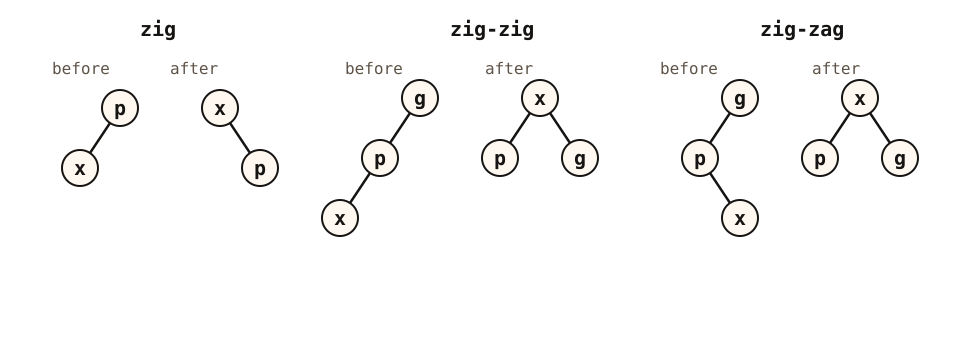
\includegraphics[width=\textwidth]{figures/rotations.svg}

The three patterns are enough:

\begin{itemize}
  \item \textbf{zig}: \(x\) has a parent but no grandparent,
  \item \textbf{zig-zig}: \(x\) and its parent are on the same side,
  \item \textbf{zig-zag}: \(x\) and its parent are on opposite sides.
\end{itemize}

The tree is not maintained by a global balance condition. Instead, the access itself reshapes the searched path.

\section*{Operations}

For ordered-set style problems, the core operations are:

\begin{itemize}
  \item \textbf{rotate(x)}: local structural change around \(x\) and its parent,
  \item \textbf{splay(x)}: repeat rotations until \(x\) becomes root,
  \item \textbf{find(key)}: BST walk, then splay the last touched node,
  \item \textbf{insert(key)}: BST insert, then splay the new node,
  \item \textbf{erase(key)}: splay the node, remove it, then join the two remaining trees,
  \item \textbf{kth(k)}: walk by subtree sizes and splay the result.
\end{itemize}

The note code keeps the ordered-set version because it shows the invariants clearly. Sequence versions usually add
lazy tags, subtree sizes, and split / merge by position.

\section*{Correctness Intuition}

The BST property is preserved because every rotation only changes the relative parent-child relation of a small
constant-size neighborhood while keeping the inorder order unchanged.

The interesting part is not correctness of one operation but why repeated splaying stays cheap on average. The rough
intuition is that splaying moves a recently useful node upward and also shortens much of the searched path around it.
Some future accesses become cheaper, and that saved work helps pay for the current restructuring.

\section*{Complexity Analysis}

One operation can still take \(O(n)\) in the worst case. The point of splay trees is the amortized bound:

\begin{itemize}
  \item search / insert / erase / split / merge: \(O(\log n)\) amortized,
  \item memory: \(O(n)\).
\end{itemize}

This is the part where the Sleator--Tarjan access lemma matters. In contest use, I mostly remember the operational
consequence: a sequence of operations is cheap even though a single one can be ugly.

\section*{Implementation}

The reference implementation keeps:

\begin{itemize}
  \item parent pointers,
  \item two children per node,
  \item subtree size,
  \item ordered-set operations on unique keys.
\end{itemize}

That is enough to exercise the full splay loop, erase-by-join, and k-th queries without burying the main idea under
sequence-specific lazy tags.

\section*{Common Pitfalls}

\begin{itemize}
  \item Forgetting to update a parent pointer during rotation.
  \item Pulling subtree sizes in the wrong order after structural changes.
  \item Splaying the wrong node after a failed search.
  \item Expecting worst-case \(O(\log n)\) instead of amortized \(O(\log n)\).
  \item Writing the base splay incorrectly, then trying to build link-cut trees on top of it.
\end{itemize}

\section*{Practice Problems}

\begin{itemize}
  \item Ordered set with insert / erase / predecessor / successor / k-th.
  \item Sequence cut-and-paste problems after upgrading to an implicit splay.
  \item Dynamic tree problems, once the splay core feels completely reliable.
\end{itemize}

\section*{References}

\begin{itemize}
  \item \href{https://zhtluo.com/cp/splay-tree-one-tree-to-rule-them-all.html}{Zhtluo: Splay Tree - One Tree to Rule Them All}.
  \item \href{https://www.cs.princeton.edu/courses/archive/fall02/cs521/ST85.pdf}{Sleator and Tarjan: Self-Adjusting Binary Search Trees}.
  \item \href{https://ocw.mit.edu/courses/6-854j-advanced-algorithms-fall-2005/cfaa2099f5edb14d32d93998efd87fc1_n3_splay.pdf}{MIT 6.854 notes on splay trees}.
\end{itemize}
